\documentclass[a4paper]{article}
\usepackage{ctex}
\usepackage{amsmath, amssymb, amsthm}
\usepackage{moreenum}
\usepackage{mathtools}
\usepackage{url}
\usepackage{bm}
\usepackage{enumitem}
\usepackage{graphicx}
\usepackage{subcaption}
\usepackage{booktabs} % toprule
\usepackage[dvipsnames]{xcolor}
\usepackage{fontspec}
\setmainfont{Times New Roman}
\usepackage{biuwork} % where the magic happens


\thecourseinstitute{中国共产党中央委员会党校}
\thecoursename{学习强国概论}
\theterm{2020 春}
\hwname{第1次作业}

% 自定义题号
\newcounter{question}[section]
\newenvironment{question}[2]
{\refstepcounter{question}\par\medskip
\noindent {\color{Cyan}\textbf{#1.} \textbf{#2}}
\par\medskip\textbf{答:}}{\medskip}

% 自动题号
% \newcounter{question}[section]
% \newenvironment{question}[1][]
% {\refstepcounter{question}\par\medskip
% \noindent \textbf{\thequestion.} \textit{#1}
% \par\medskip\textbf{答:}}{\medskip}

\begin{document}
\courseheader
\name{晓芬红}{2020031415}

\begin{question}{1}{毛泽东思想活的灵魂的三个基本方面是什么?}
    \begin{enumerate}
        \item 实事求是
        \item 群众路线
        \item 独立自主
    \end{enumerate}
\end{question}

\begin{question}{3}{Which of the OSI layers and TCP/IP layers handles each of the following:
    \\1) Dividing the transmitted bit stream into frames
    \\2) Determining which route through the subnet to use.}
        \begin{center}
        \begin{tabular}{ |c|c|c| }
        \hline
        - &把传输的比特流分成帧 & 确定使用哪条路由来通过子网\\
        \hline
        OSI & 数据链路层 & 网络层 \\
        TCP/IP & 链路层 & 互联网层 \\
        \hline
        \end{tabular}
        \end{center}
\end{question}

\begin{question}{*10}{As a simplistic example, suppose that time is divided into discrete slots, with each of the n hosts attempting to use the channel with probability p during each slot. What fraction of the slots will be wasted due to collisions?}
    设冲突概率为$P_{collisions}$,空闲概率为$P_0$,一台主机使用的概率为$P_1$,则
    \[P_0=\binom{N}{0}\times p^0\times (1-p)^n=(1-p)^n\]
    \[P_1=\binom{N}{1}\times p^1\times (1-p)^{n-1}=n\times p\times(1-p)^{n-1}\]
    而冲突时间比例即为冲突概率,即为:
    \[P_{collisions}=1-P_0-P_1=1-(1-p)^n-n\times p\times(1-p)^{n-1}\]
\end{question}

\begin{question}{35}{. Try using ping to see how long it takes to get from your location to several known locations.}
    LOL, good question.\\
    Ping mit.edu and then use Wolframalpha find the distance between LA and MIT:
    \begin{center}
        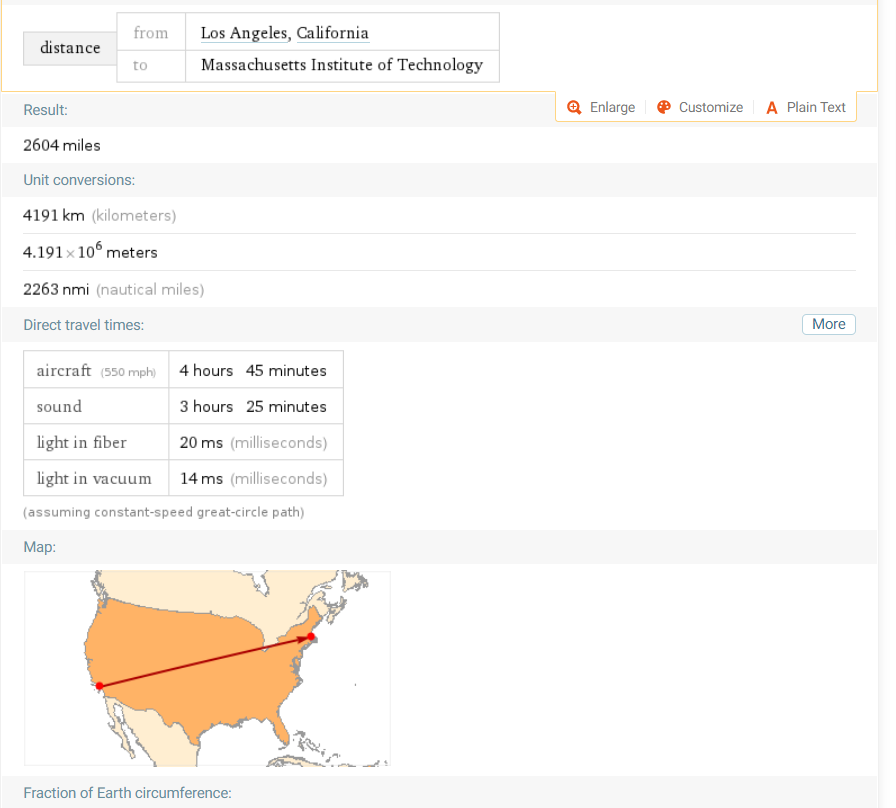
\includegraphics[width=.9\textwidth]{images/la-mit.png}
    \end{center}
    and ...
\end{question}

\end{document}
